\section{Background}\label{sec:bak}

\begin{figure}[t]%
    \centering
    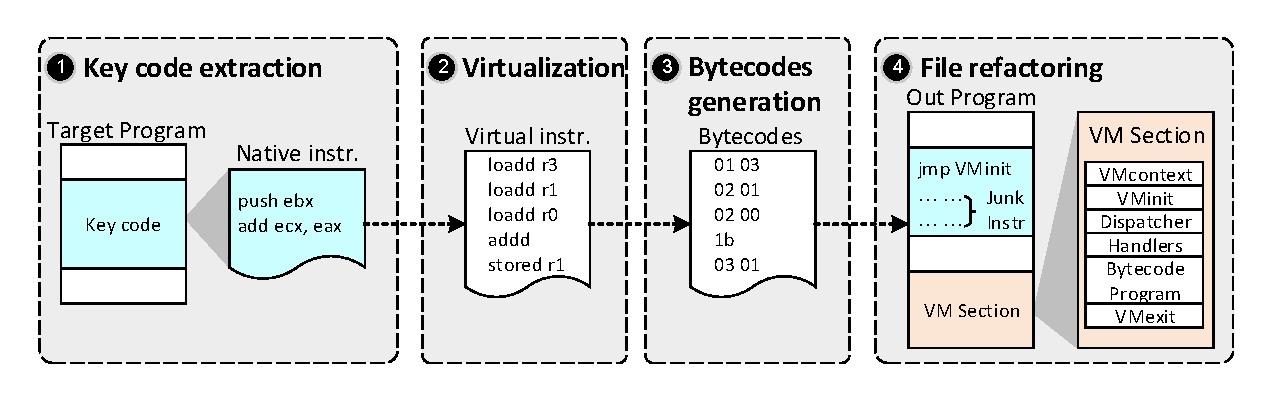
\includegraphics[width=1\columnwidth]{figure/figvmp.pdf}
    \caption{A classical process for VM-based code obfuscation. 
    To obfuscate the code, we first dissemble the code region to be protected into native assembly code (1). The assembly code will be mapped
    into our virtual instructions (2) which will then be encoded into a bytecode format (3). Finally, the generated byecode will be inserted into a specific region of the binary which is linked with a VM library (4).
    }\label{fig:Fig.vmp}
    %\vspace{-5mm}
\end{figure}

\subsection{VM-based Code Obfuscation}
VM-based code obfuscation often performs at the binary level for an already
compiled program. As shown in Figure~\ref{fig:Fig.vmp}, the obfuscation
process typically follows a number of steps. Firstly, the critical code
segment to be protected will be extracted from the compiled binary, which
will be dissembled into assembly code. Next, the native assembly code will
translated into virtual instructions (a machine-independent intermediate
representation used by our VMs) which are functional equivalent to original native code.
Then, the generated virtual instructions will be encoded into the bespoke
bytecode format.  Finally, a new VM section will be linked (or inserted) into
the target program where the entry point of the protected code region will be
redirected to a function call to invoke the VM to translate the bytecode
instructions to native machine code at runtime. The idea of VM-based code
obfuscation is to force the attacker move from a familiar
instruction set (e.g. x86) to an unfamiliar bespoke virtual instruction set,
which hopefully will significantly increase the time and efforts for 
reverse-engineering. 


\subsection{VM Components.} Our approach follows a classic VM implementation,
consisting of a number of components that are shown
in step 4 at Figure~\ref{fig:Fig.vmp}.
The context of the native program, which includes
information such as local variables, function arguments, the return address etc.,
will be stored in a register-based VM memory space called \texttt{VMContext}. When entering the VM, the \texttt{VMinit}
component saves the native program context and initializes the
\texttt{VMContext}. After executing the protected code segment,  \texttt{VMExit} restores the
native program context, and then returns the program control back to the
original program to continue executing the rest of the program.
At the heart of the VM is an interpreter consisting of a
dispatcher and a handler set described as follows. The dispatcher fetches a
bytecode that is ready to be exeucted, decoding the fetched
bytecode (by parsing the opcode and the operand), and then assigning a handler (from a collection of handlers that can be used
to interpret the bytecode)  to translate the fetched bytecode to native
machine code. This process iterates until all the bytecode are executed.
For the attacker's perspective, the key to understand the
logic of the protected code region is to find out how
bytecode or virtual instructions are mapped into native machine code.

\begin{figure}[t]%
    \centering
    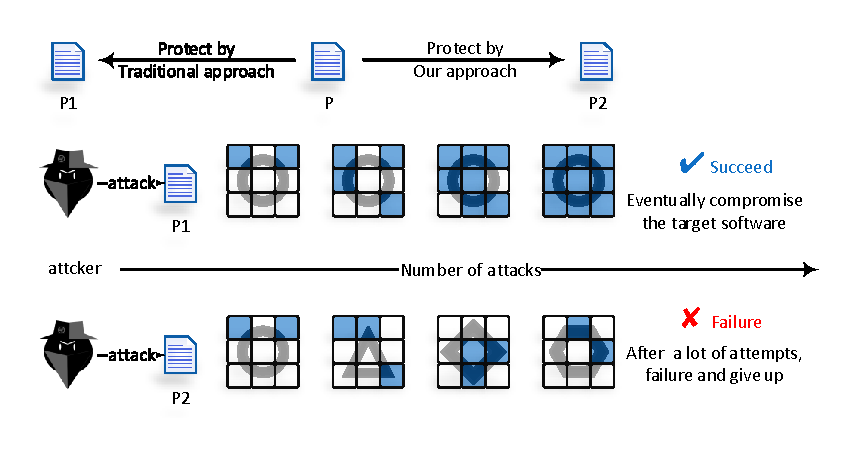
\includegraphics[width=0.7\columnwidth]{figure/figattack.pdf}
    \caption{Diversity affects the attack effectiveness. In this example, a dark small square represents reusable attacking knowledge. Diverse program execution increases the difficulty for performing reverse-engineering based attacks.}\label{fig:Fig.attack}
    %\vspace{-5mm}
\end{figure}

\subsection{The Design Goal}
As a motivation example, consider Figure~\ref{fig:Fig.attack} that illustrates how an attacker
can reuse knowledge extracted from the previous runs of the same application or
other applications that are protected using the same VM scheme to perform an reverse-engineering attack.
This kind of attacks is referred as \emph{cumulative attacks} in this paper.
In the first scenario, the software always follows the same execution path
across multiple runs. Under this setting, the attacker may be able to use a few runs to
obtain sufficient knowledge about the program behavior.
In the second scenario, the program execution path changes across different runs.
As such, it will take longer and many more runs to gather enough information to perform the attack.
As can be seen from this simple illustration, diversity is key for us to protect software against dynamic cumulative attacks.
This is the aim of this work, to improve the diversity of program executions for code obfuscation.
It is to note that like any other code protection techniques, our approach could be exploited by malware.
How to prevent this is out of the scope of this work.
